%%%% début de la page
\teteSndMouv

%%
\nomPrenomClasse


%%%% titre
\numeroActivite{5}
\titreActivite{Forces d'interaction gravitationnelle}


%%%% objectifs
\begin{objectifs}
  \item Connaître la force d'interaction gravitationnelle
\end{objectifs}


%%%% evaluation
\begin{tableauCompetences}
  COM & Travailler en groupe, échanger entre élèves. & & & &
\end{tableauCompetences}


%%
\begin{doc}{Force d'interaction gravitationnelle}{doc:A5_interaction_gravitationnelle}
  \chevron Tous les corps qui possèdent une masse s’attirent entre eux : c’est l’attraction gravitationnelle.

  \begin{encart}
    On modélise l'attraction gravitationnelle exercée par le corps $A$ sur le corps $B$ par une force représentée par un vecteur $\vvFAsurB$ :
    
    \vspace*{-12pt}
    \begin{wrapfigure}[6]{r}{0.4\linewidth}
      \vspace*{-20pt}
      \begin{tikzpicture}
        % corps A
        \tkzCercle{0}{0}{gray!50!white}{20}
        \tkzLabel{-1.2}{0}{$m_A$}
        \tkzPointLabel{0}{0}{$A$}
        % corps B
        \tkzCercle{4}{2}{gray!50!white}{20}
        \tkzLabel{2.8}{2}{$m_B$}
        \tkzPointLabel{4}{2}{$B$}
        % force et distance
        \tkzVecteur(4)[-1.75](2)[-0.875]{$\vvFAsurB$}[left]
        \tkzVecteur(0.5)[4](-1)[2]{}*
        \tkzLabel{2.5}{-0.5}{$d$}
      \end{tikzpicture}
    \end{wrapfigure}

    \phantom{b}
    \begin{listePoints}
      \item \important{Point d'application} : centre du corps $B$
      \item \important{Direction} : la droite $AB$.
      \item \important{Sens} : de $B$ vers $A$ (force attractive).
      \item \important{Valeur} : 
    \end{listePoints}
    \begin{center}
      $\FAsurB =$ \texteTrouLignes{$G\times \dfrac{m_A \times m_B}{d^2}$}
    \end{center}
      
    Dans la formule de la valeur de la force, les masses s'expriment en kilogramme (\unit{\kg}),
    la distance en mètre (\unit{\m}) et
    la \important{constante universelle de gravitation $\mathbf{G}$} en newton mètre carrée par kilogramme carrée (\unit{\newton \m\squared \per\kg\squared}).
    Sa valeur (à connaître) est 
    \begin{center}
      $G =$ \texteTrou{$\qty{6,67e-11}{\newton \m\squared \per\kg\squared}$}
    \end{center}
  \end{encart}
\end{doc}

%%%%
\numeroQuestion Compléter le document \ref{doc:A5_interaction_gravitationnelle}.


\question{
  Donner des exemples d'actions mécaniques qu'on peut rencontrer dans la vie quotidienne.
}{

}{5}

\question{
  Quelle différence remarquez-vous entre ces actions de la vie quotidienne et l'interaction gravitationnelle ?
}{

}{3}


%%%%
\begin{doc}{Satellite Hubble}{doc:A5_satellite_hubble}
  \begin{wrapfigure}{r}{0.3\linewidth}
    \vspace*{-24pt}
    \centering
    \image{1}{images/mecanique/hubble}
  \end{wrapfigure}
  
  Le satellite Hubble est un satellite de masse $m_H = \qty{1,1e4}{\kg}$ conçu par la NASA avec une  participation de l'Agence spatiale européenne, l'ESA.
  
  Le satellite est attirée par la terre : il est en chute libre permanente.
  Le satellite est opérationnel depuis 1990 et tourne autour de la Terre en \qty{96}{\min}.
  Vu depuis le centre de la Terre, il a un mouvement circulaire uniforme à une altitude $\mathbf{h = \qty{590}{\km}}$.
  
  Ce satellite contient un télescope qui permet d’observer les étoiles et objets de l’univers depuis l’espace !
\end{doc}

\mesure 
Sur le schéma ci-dessous, représenter la force d’interaction gravitationnelle $F_{T/H}$ exercée par la Terre $T$ sur le satellite Hubble $H$.
La Terre est assimilée à une boule de rayon $R_T = \qty{6,37e3}{\km}$ et de masse $M_T = \qty{5,97e24}{\kg}$.

\begin{center}
  \begin{tikzpicture}
    % Terre et Satellite
    \tkzCercleLigne{0}{0} {white}{couleurSec} {80}
    \tkzCercleLigne{0}{0} {couleurPrim!30}{couleurPrim} {50}
    \tkzPointLabel{2}{2}{$H$}
    \tkzPointLabel{0}{0}{$T$}
    % Distance
    \tkzVecteur(0)[-2.8](0){$d$}[below right]*
    \tkzVecteur(0)[-1](0)[-1.48]{}*
    \tkzLabel{-0.3}{-1}{$R_T$}
    \tkzVecteur(-1)[-0.6](-1.48)[-0.88]{}*
    \tkzLabel{-1.}{-2}{$h$}
  \end{tikzpicture}
\end{center}



\question{
  Donner la formule mathématique qui relie la valeur de la force $F_{T/H}$ et la masse du satellite $m_H$, la masse de la Terre $M_T$, la constante $G$ et la distance $d$.
}{

}{3}

\question{
  Exprimer $d$ en fonction de $R_T$ et $h$.
  Calculer la valeur de $d$ en mètre.
}{

}{2}

\question{
  Calculer la valeur de $F_{T/H}$.
}{

}{4}